\documentclass{article}


\usepackage{conference}

\usepackage[utf8]{inputenc} % allow utf-8 input
\usepackage[T1]{fontenc}    % use 8-bit T1 fonts
\usepackage{hyperref}       % hyperlinks
\usepackage{url}            % simple URL typesetting
\usepackage{booktabs}       % professional-quality tables
\usepackage{amsfonts}       % blackboard math symbols
\usepackage{nicefrac}       % compact symbols for 1/2, etc.
\usepackage{microtype}      % microtypography
\usepackage[final]{graphicx}% graphics
\usepackage{lipsum}

\title{Retour vers le \emph{cosmos}}
%{F.M. Sanchez,\ M. Grosmann,\ B. Kress,\ N. Flawisky,\ L. Gueroult, \textit{Cosmic Holography}}
\author{
  F.M. Sanchez~hol137\thanks{Retired Professor} \\
  Department of Physics\\
  Paris 11 University\\
  Paris, FRANCE \\
  \texttt{hol137@yahoo.fr} \\
  %% examples of more authors
   \And
 M.H. Grosmann\thanks{Retired Professor} \\
  Department of Photonics\\
  University of Strasbourg\\
  Strasbourg, FRANCE \\
  \texttt{michel.grosmann@me.com} \\
   \And
 D. Tassot\thanks{Retired Professor} \\
  Ecole des Mines\\
  %University of Strasbourg\\
  %Strasbourg, FRANCE \\
  \texttt{tassot@me.com} \\
  %% \AND
  %% Coauthor \\
  %% Affiliation \\
  %% Address \\
  %% \texttt{email} \\
  %% \And
  %% Coauthor \\
  %% Affiliation \\
  %% Address \\
  %% \texttt{email} \\
  %% \And
  %% Coauthor \\
  %% Affiliation \\
  %% Address \\
  %% \texttt{email} \\
}


\begin{document}
\maketitle

\begin{abstract}
%\lipsum[1]
Le modèle du ”Big-Bang”, le modèle ”Cosmhologique”, les radars de la police et les taupes très myopes !
\end{abstract}


% keywords can be removed
\keywords{Quantum \and Holography \and Cosmos}


\section{Introduction}

Le modèle dit du Big-Bang est une description de l'origine et de l'évolution de l’Univers datant du début du 20éme siècle.

De façon générale, le terme « Big Bang » est associé à toutes les théories qui décrivent notre Univers comme issu d'une dilatation rapide. Par extension, il est également associé à cette époque dense et chaude qu’aurait connue l’Univers il y a 13,8 milliards d’années, (sans que cela préjuge forcément de l’existence d’un « instant initial » ou d’un commencement à son histoire).

\section{Le modèle du ”Big-Bang”}
\label{sec:headings}

Le terme a été initialement proposé en 1927 par l'astrophysicien  et chanoine catholique belge Georges Lemaître, qui décrivait dans les grandes lignes l’expansion de l'Univers, plus précisément décrite par l'astronome américain Edwin Hubble en 1929. Ce modèle fut désigné pour la première fois sous le terme ironique de « Big Bang » lors d’une émission de la BBC, The Nature of Things en 1949 (dont le texte fut publié en 1950), par le physicien britannique Fred Hoyle. Lui-même préférait les modèles d'état stationnaire.

%Voir Section \ref{sec:headings}.

\subsection{Concept General}
%\lipsum[5]
Le concept général du Big Bang, à savoir que l’Univers est en expansion et a été plus dense et plus chaud par le passé, doit sans doute être attribué au Russe Alexandre Friedmann, qui l'avait proposé en 1922, cinq ans avant Lemaître. Son assise fut cependant considérée comme mieux établie en 1965 avec la découverte du fond diffus cosmologique. Georges Lemaître le qualifia d’« éclat disparu de la formation des mondes, attestant de façon définitive la réalité de l’époque dense et chaude de l’Univers primordial ». Albert Einstein, en mettant au point la relativité générale, aurait pu déduire l'expansion de l'Univers, mais a préféré modifier ses équations en y ajoutant sa constante cosmologique, car il était persuadé que l'Univers devait être statique.

Le terme de « Big Bang chaud » (« Hot Big Bang ») est parfois utilisé initialement pour indiquer que, selon ce modèle, l’Univers était plus chaud quand il était plus dense.

\subsubsection{Partisans et adversaires: la controverse}
%\lipsum[6]

Partisans et adversaires du modèle du Big Bang.

Dès le début, ce modèle fut jugé séduisant par tous les amateurs d'un concept de « création » de l'Univers. Mais les tenants de l'énoncé attribué à Lavoisier : « Rien ne se perd, rien ne se crée ! Tout se transforme ! », réagirent dès le début négativement à la proposition. 

Par ailleurs de grandes critiques furent présentées sur les évaluations numériques de l'espace et du temps aux grandes distances envisagées : Dans ce modèle, les mesures de temps et d'espaces sont les unes et les autres basées sur le « décalage spectral » dû à l'effet Doppler. Dans le principe ceci ressemble à la mesure par les radars de la police de la vitesse des véhicules : 

Si un objet vibrant à une fréquence f1 s'éloigne de nous avec une vitesse V, nous le percevons (à cause de la vitesse limitée de la lumière) comme vibrant avec une fréquence f2 plus petite, (on dit «  décalée vers le rouge »). La mesure de la différence Df = f1 – f2 permet d'évaluer la « vitesse d'éloignement » de l'objet par rapport à l'observateur. 

%\lipsum[7]
Pour les « objets célestes » proches de nous on peut mesurer les positions et les vitesses par triangulation. Des mesures expérimentales permirent de comparer les valeurs de distances et vitesses obtenues par triangulation et les valeurs de «  décalage spectraux ». Hubble et Humason constatèrent une proportionnalité entre les valeurs des positions et des vitesses et présentèrent cette proportionnalité (« Lois de Hubble ») comme une observation expérimentale. Mais cette proportionnalité découle naturellement du fait que ces valeurs sont respectivement obtenues en multipliant le décalage Df par un coefficient A pour la première et B pour la seconde ! Elle est donc simplement le quotient de A par B !

Pour les objets célestes trop éloignés pour permettre des mesures géométriques des distances et des vitesses une autre méthode d'évaluation fut découverte : des objets célestes, les « céphéides » présentent une luminosité qui varie périodiquement. La mesure de la fréquence correspondante permet une « autre évaluation » de la distance et de la vitesse. Elle semble confirmer le modèle du BIG-BANG.

Mais elle est aussi basée sur le principe de l'effet Doppler. Et a le même défaut que la première : Il est bien difficile de discriminer entre « décalage dû à un déplacement longitudinal » et « décalage dû à un déplacement transversal ».

Les partisans du BIG-BANG expliquent qu'il n'y a « que des déplacements longitudinaux ».

Leurs adversaires rétorquent que « justement cela reste à démontrer » et que les données expérimentales permettent d'envisager une « Univers en rotation » aussi bien qu'un « Univers en expansion » …

Depuis bientôt un siècle, les controverses ne font que s'amplifier. La Science-Fiction a inspiré de nouvelles idées et concepts sur les « temps » et les « espaces » : virtualités, multivers, trous de vers, etc …

\section{Le ”modèle Cosmhologique"}
\label{sec:headings}

Dans ce modèle il n'y a pas de « début » ni de « fin » de l'Univers.

D'une part il est vraisemblable que le développement des techniques expérimentales et de l'amélioration corrélative des théories en optique (LASERs, Optiques Holographiques, Photonique, etc… ) va peut-être prochainement permettre de très grandes améliorations en observations. De nouvelles données expérimentale sont recueillies tous les jours par quantité d'instruments qui n'existaient pas il y a quelques années

D'autre part des considérations théoriques nouvelles essaient de prendre en compte ces nouveaux résultats. Les unes pour les intégrer dans des théories existantes. D'autres pour servir de bases à de nouvelles théories. 

Le ”modèle Cosmhologique” (développé par l’équipe du professeur Francis Sanchez) en est un exemple : Il suppose un Univers Visible limité par la vitesse de la lumière mais intégré dans un Univers plus vaste. 

On peut faire l'analogie avec une taupinière, au sommet de laquelle des taupes très myope et qui ne voient pas jusqu'à la base de la taupinière, ont imaginé un Univers limité au sommet de leur taupinière. Mais qui, développant des instruments, leur permettant d'agrandir leur champ de vision, découvrent petit à petit, qu'au bas de la taupinière existent peut-être des « choses » (terre, brins d'herbe etc …) qu'elles essaient de se représenter … en polémiquant entre elle sur les différents « modèles » possibles …

En appliquant les principes de la thermodynamique (qui font déjà polémiques au niveau de la planète et du réchauffement climatique) à l'Univers, il est possible d'imaginer un Univers cyclique de très grandes dimensions.

Il serait composée de deux parties : l'une visible ”tardionique” à « courte » portée … L'autre « tachyonique » à bien plus grande échelle !

Ce modèle permet de réconcilier les contradictions entre MACRO- et micro- Physiques et évite les paradoxes de « matière noire et « énergie noire » qui handicapent les modèles de type Big-Bang …

Certaines vérifications expérimentales pourront être prochainement effectuées par des satellites en projet et par des expériences, lors du redémarrage dans 2 ans du CERN à Genève.


\section{Conclusions}
\label{sec:headings}

Les récentes découvertes expérimentales en macro- et micro- Physique permettent d'imaginer un modèle d'Univers qui résoudrait élégamment les contradictions actuelles entre ces deux sous-disciplines. De nouvelles expériences (en préparation) devraient permettre de confirmer la pertinence de ce modèle face aux très nombreux autres actuellement en compétition. Nous essayons actuellement de le représenter sous forme d'un hologramme. Dans la conception de celui-ci nous avons réalisé des stéréoscopies dont l'une est présentée sur la Figure.

On y voit la représentation (étonnement sous forme d'une droite!) de divers paramètres tant de la MACRO- que de la micro- Physique.


\subsection{Figures}

Voir Figure \ref{fig:figure_label}. Pour plus d'explications. \footnote{http://vixra.org/abs/1904.0218}
 

\begin{figure}
  \centering
  %\fbox{\rule[-.5cm]{4cm}{4cm} \rule[-.5cm]{4cm}{0cm}}
  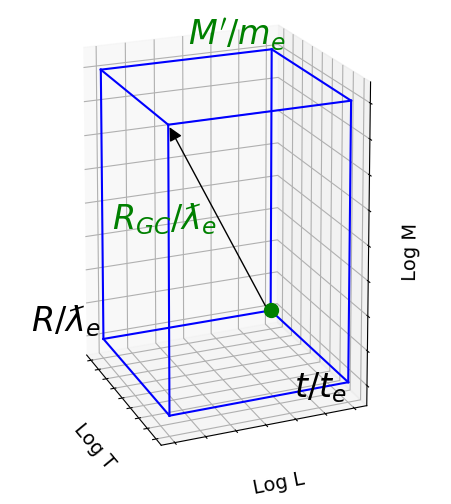
\includegraphics[width=15cm,height=16cm]{./figures/triaxis.png} 
  \caption{Representation Geo dimensionelle du couple Univers-Grandcosmos. Dans un super espace 3D, les logarithmes naturels de temps, de longueurs et de masses sont consideres comme vecteurs. Le rapport logarithmique du rayon du grand cosmos avec la longueur d'onde de l;electron Compton fait apparaitre un vecteur norme projetant longueur et temps avec une proportion commune; le rayon de Hubble par la longueur d;onde de l'electron Compton et pour le rapport de masse; on considere $M^{\prime}$ par la masse de l'electron. $M^{\prime}$ etant la masse critique dans le Grandcosmos reduit a un hologramme spherique, ceci demontre la confirmation geometrique du principe holographique etendu (2D-1D)applique a l'univers d'entropie de Bekenstein Hawking. L'existence d'un grand cosmos ne peut plus etre niee depuis que la relation entre $e$, $a$ et les logarithmes impliques atteignent une precision de $10^{-7}$.}
  \label{fig:figure_label}
\end{figure}


\subsection{Lists}
\begin{figure}
  \centering
  %\fbox{\rule[-.5cm]{4cm}{4cm} \rule[-.5cm]{4cm}{0cm}}
  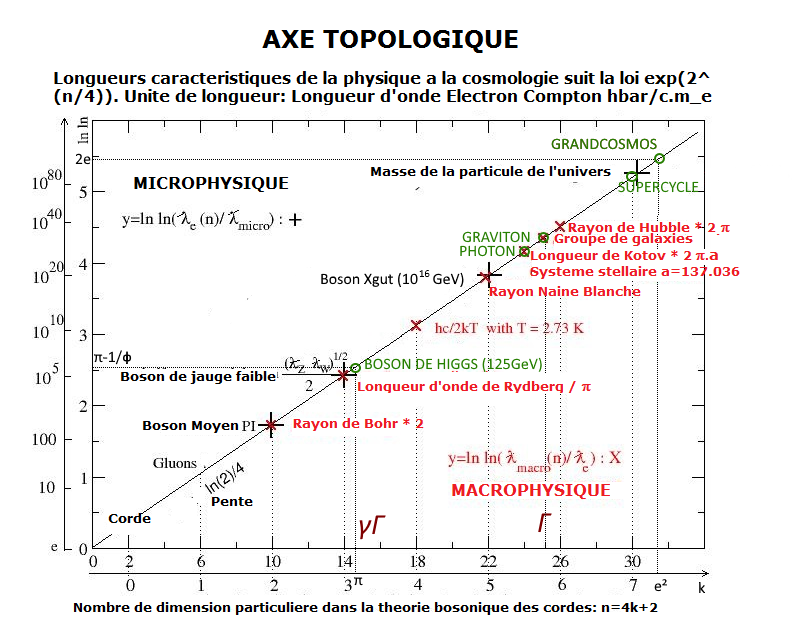
\includegraphics[width=15cm,height=16cm]{./figures/figure.png}
  \caption{L'axe topologique. Le double logarithme naturel (y = lnln(Y)) de quantites physique sans dimensions 
(Y) corresponds a la corde dimensionelle de series n = 4k + 2, de k = 0 a k = 7, montrant la periodicite de Bott qui est a l'origine du nom Axe Topologique.}
  \label{fig:figure_label}
\end{figure}
\begin{itemize}
\item Axe Topologique
\end{itemize}


\bibliographystyle{unsrt}  
%\bibliography{references}  %%% Remove comment to use the external .bib file (using bibtex).
%%% and comment out the ``thebibliography'' section.


%%% Comment out this section when you \bibliography{references} is enabled.
\begin{thebibliography}{1}

\bibitem{Sanchez3} Sanchez F.M. ``Towards the grand unified Holic Theory''. Current
Issues in Cosmology. Ed. J.-C. Pecker and J. Narlikar. Cambridge Univ. Press,
2006; p. 257--260.

\bibitem{Sanchez4} Sanchez F; M. ``Holic Principle: The coherence of the Universe`` (Sept 1995), Entelechies, 16th ANPA, 324--344.
\bibitem{Grosmann} Grosmann, M. and Meyrueis P. ``Optics and Photonics Applied to Communication and Processing''. SPIE.  Jan 1979.
\newblock Optics and Photonics Applied to Communication and Processing.
\newblock In {\em SPIE (SPIE), 1979 
  International Conference on}, pages . SPIE, 1979.
\bibitem{Grosmann2} Grosmann, M and Rebordão, José and Meyrueis, Patrick, 1985,02,p761--765,Propagation Of Waves In Optical Systems: Reformulation Of Huyghens Principle For Aspheric Systems,
volume 491, Proceedings of SPIE - The International Society for Optical Engineering, doi:10.1117/12.968010
\bibitem{Kress} Digital Diffractive Optics: An Introduction to Planar Diffractive Optics and Related Technology, by B. Kress, P. Meyrueis, pp. 396. ISBN 0-471-98447-7. Wiley-VCH , October 2000.
\newblock An Introduction to Planar Diffractive Optics and Related Technology.
\bibitem{Sanchez5} F.M. Sanchez, V. Kotov, M. Grosmann, D. Weigel, R. Veysseyre, C. Bizouard, N. Flawisky, D. Gayral, L. Gueroult, Back to Cosmos
\newblock {\em arXiv preprint viXra:1904.0218}, 2019.
\end{thebibliography}
\begin{appendix}

%This is the appendix section

%\subsection{Glossary}

%This is the glossary section for the definition of the terms used in this paper.

\begin{description}
\item Antimatière (re-définition): matière qui oscille en opposition de phase avec la matière
environnante
\item Big-Bang: Hoyle who was the first to introduce the term Big Bang in Cosmology never believed in such a theory. 
\item Black Hole
\item Cosmos: ensemble de tout ce qui existe.
\item Grand Cosmos:
\item Gluonde
\item Hol: 
\item Holic:
\item Immergence (néologisme) Faculté du tout à expliquer les parties. S’oppose à la
classique ‘émergence’, qui attribue à un ensemble des propriétés nouvelles,
étrangères à celles de ses éléments constitutifs.
\item Infini (obsolète) concept inventé par les formalistes pour simplifier certains calculs,
notamment les séries.
\item Matière noire : matière qui oscille en quadrature de phase avec la matière
environnante
\item Mur de Planck (obsolète) : limite spatio-temporelle officielle. La cosmologie
Cohérente le repousse d’un facteur $10^{61}$, résolvant ainsi l’énigme de la densité du
vide quantique, $10^{122}$ fois l’énergie moyenne cosmique.
\item Neutrons : particules remontant l’organisation de l’Univers, en apparaissant dans les
espaces inter-sidéraux, à raison d’un neutron par siècle dans le volume d’une
cathédrale.
\item Observable Universe
\item Permanent Big bang
\item Photonde (néologisme): désigne l’onde associée à un photon, quantum d’énergie qui
disparaît d’un atome émetteur pour se retrouver sur un atome récepteur, après un
calcul cosmique.
\item Rayonnement thermo-cosmique rayonnement interne du Cosmos. Appelé CMB
(Cosmic Microwave Background) par la science pré-science.
\item Rayon critique : rayon de chaque univers particulaire. Il s’identifie avec le ‘rayon de
Hubble’ directement mesurable. C’est aussi le Rayon de Schwarzschild de chaque
Univers particulaire considéré comme un trou noir dont la particule est la singularité
centrale.
\item Schwarzschild radius
\item Tachyon: particule se déplaçant plus vite que la lumière. Il a été exclu par la
préscience.
\item Toponde
\item Trou noir : miniaturisation d’un univers particulaire. Les trous noirs ont pour fonction
d’évacuer la matière interne d’un amas galactique.
\item Univers: l’écume immergente du Cosmos, $10^122$ fois moins énergétique
\item Univers particulaire (néologisme) : partie de l’Univers qui construit et déconstruit
chaque particule.
\item Visible Horizon:
\item White Hole
\end{description}



Principe Conceptuel (néologisme) : Le Cosmos est ordonné par des lois esthétiques,
compréhensibles par les humains. Il remplace le Principe anthropique officiel, mal
défini et objet de graves contre-sens.

Science (re-définition) : connaissance des lois du Cosmos.
Préscience (néologisme) connaissances partielles hors cosmos.
Variables cachées (obsolète) : dans la préscience, causes invoquées pour expliquer
l’Univers. Elles s’identifient au Cosmos.
Vide quantique : partie principale du Cosmos.

Univers particulaire (néologisme) : partie de l’Univers qui construit et déconstruit
chaque particule.
Intrication (ou Non-séparabilité) : manifestation de l’ordonnancement cosmique entre
les univers particulaires
Tachyon : particule se déplaçant plus vite que la lumière. Il a été exclu par la
préscience.
Infini (obsolète) concept inventé par les formalistes pour simplifier certains calculs,
notamment les séries.
Nombre réel (trompeur et obsolète) type de nombre inventé par les mathématiciens
formalistes, mais qui interdit tout calcul pratique, donc cosmique.
Cosmologie cohérente (néologisme) : cosmologie où tous les Univers particulaires
sont équivalents. S’oppose au Multivers disparate officiel qui attribue des propriétés
différentes à une série indéfinie et non observable d’univers.
Principe Cosmologique Parfait (re-définition) : chaque Univers particulaire est
globalement homogène, isotrope et invariant.

Récession galactique : répulsion entre amas de galaxies permettant de renouveler
l’Univers au profit de nouveaux neutrons

Big bang (re-définition) phase de reconstruction d’un univers particulaire. Dans la
cosmologie cohérente il est permanent
Big crush (re-définition) phase de déconstruction d’un univers particulaire
Chronon (néologisme): atome insécable de temps, entre un bang et un crush
Topon : (néologisme) atome insécable d’espace
Quantinuum (néologisme) : ensemble d’états discrets, par opposition au continuum.Continuum (obsolète) idéalisation des formalistes, rendant toute compréhension
impossible.


Principe Holographique principe expliquant la structuration du Cosmos en identifiant
des variétés topologiques de différentes dimensions. Il relie l’énormité du cosmos, à
partir de la quantification nécessaire de la constante d’Archimède pi.
Axe Topologique : ordonnancement des structures principales du Cosmos.
Equation Diophantienne équation portant sur des nombres entiers
Principe Holique Idéalisation diophantienne du Principe Holographique
Photonde (néologisme): désigne l’onde associée à un photon, quantum d’énergie qui
disparaît d’un atome émetteur pour se retrouver sur un atome récepteur, après un
calcul cosmique.
Gravitonde (néologisme): désigne l’onde associée à un graviton, quantum d’énergie
qui disparaît d’un atome émetteur pour se retrouver sur un atome récepteur après un
calcul cosmique.
Inertie Reconstitution cosmique d’un objet et de son mouvement par rapport au
Cosmos
Référentiel d’inertie tout référentiel en mouvement linéaire dans le Cosmos. La pré-
science était incapable de le définir.
Vitesse absolue : vitesse par rapport au Cosmos. La vitesse absolue du groupe local
est de $620 km/s$.Dé-synchronisation : décalage temporel provoqué lors d’un déplacement, provoqué
par déphasage dans le processus de reconstruction.
Groupe local : groupe de galaxies contenant la Galaxie, notre voie lactée.
Rayonnement thermo-cosmique rayonnement interne du Cosmos. Appelé CMB
(Cosmic Microwave Background) par la science pré-science.
\end{appendix}
\end{document}
